\section{Optimization problem \& Unconstrained optimization}

\begin{frame}{Optimization problem in general}
    \begin{itemize}
        \item Formally, an optimization problem in general (or abstract) form:
        \begin{equation}
            \underset{\text{s.t. } x \in \omega}{\min}f(x)
        \end{equation}
        \item A point that minimizes $f$ over $\Omega$
        \begin{equation}
            f(x) \geq f(x^*), \forall x \in \Omega
        \end{equation}
        \begin{itemize}
            \item Maybe not exists!
            \item Or maybe not unique!
        \end{itemize}
    \end{itemize}    
\end{frame}

\begin{frame}{Unconstrained optimization problem}
    \begin{itemize}
        \item Constraint set (or feasible set): $\Omega = \R^n$
        \item Decision variables are not constrained at all. The goal is only to minimize the objective function.
    \end{itemize}
\end{frame}

\begin{frame}{Application of Unconstrained optimization problem}
    One popular application and its real-world applied situation:
    \begin{itemize}
        \item Application: Least square
        \item Real-world application: Data fitting
    \end{itemize}
    Problem statement:
    \begin{itemize}
        \item Input: $A$ be $m \times n$ matrix, $b$ be vector $m \times 1$
    \end{itemize}
    Solve:
    \begin{equation}
        \underset{x}{\min}\|Ax - b\|
    \end{equation}
\end{frame}

\begin{frame}{Application of Unconstrained optimization problem}
    \begin{figure}[h!]
        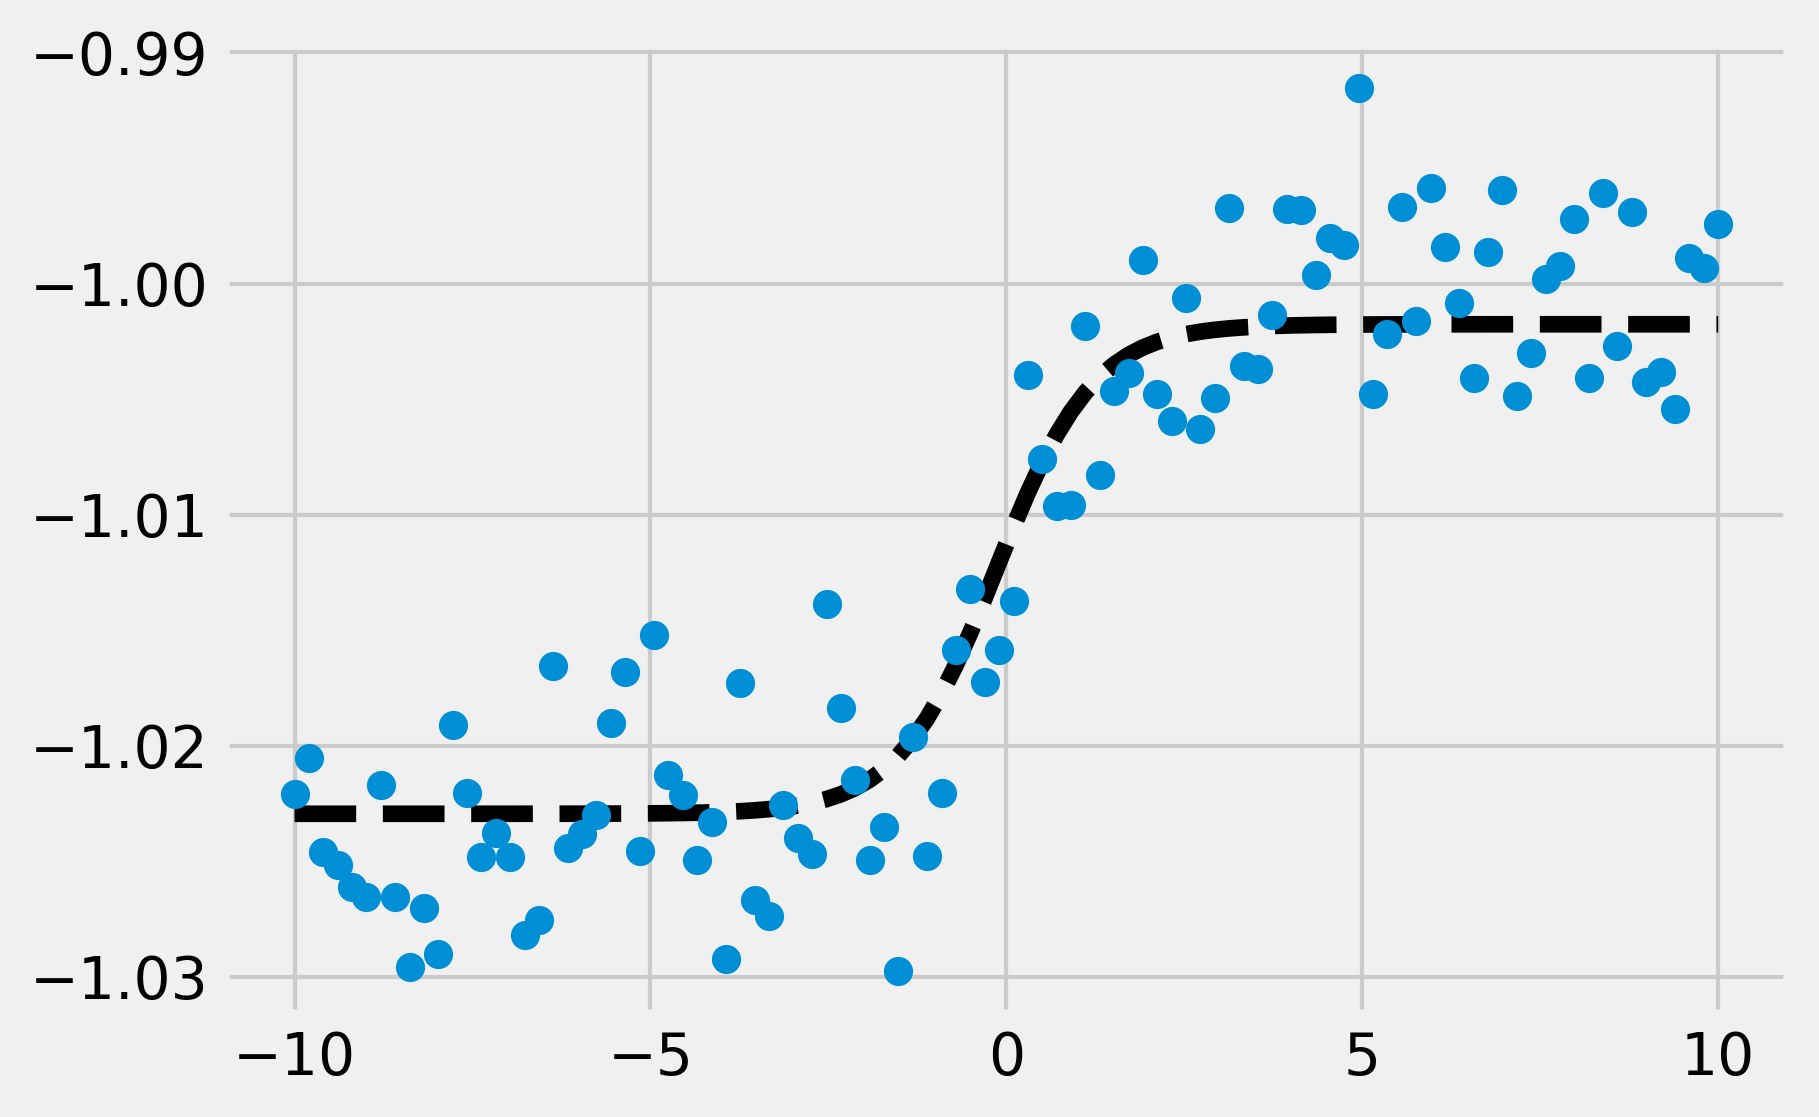
\includegraphics[width=0.55\linewidth]{figures/03_curvefitting_14_0.png}
        \caption{Example data fitting.}
    \end{figure}
\end{frame}